% Tutorial 02

\subsection{Tutorial 2: Double decoupling method \& corrections for net-charge changes}
The double decoupling method (DDM)~\cite{DDM} is an alchemical perturbation approach to compute binding free energies from molecular dynamics simulations by making use of a thermodynamic cycle (Figure \ref{TC_ASA}). Two of the branches are determined by thermodynamic integration corresponding to the decoupling of the ligand from the system (perturbing the ligand into a non-interacting dummy molecule), free in solution and when bound to the host. In order to avoid sampling of non-relevant phase space in the complexed system, the ligand is kept in a position that resembles that of the native bound conformation by gradually introducing a harmonic distance restraint. The free energy of the restraint removal can be evaluated analytically.

\begin{figure}[H]
    \centering
    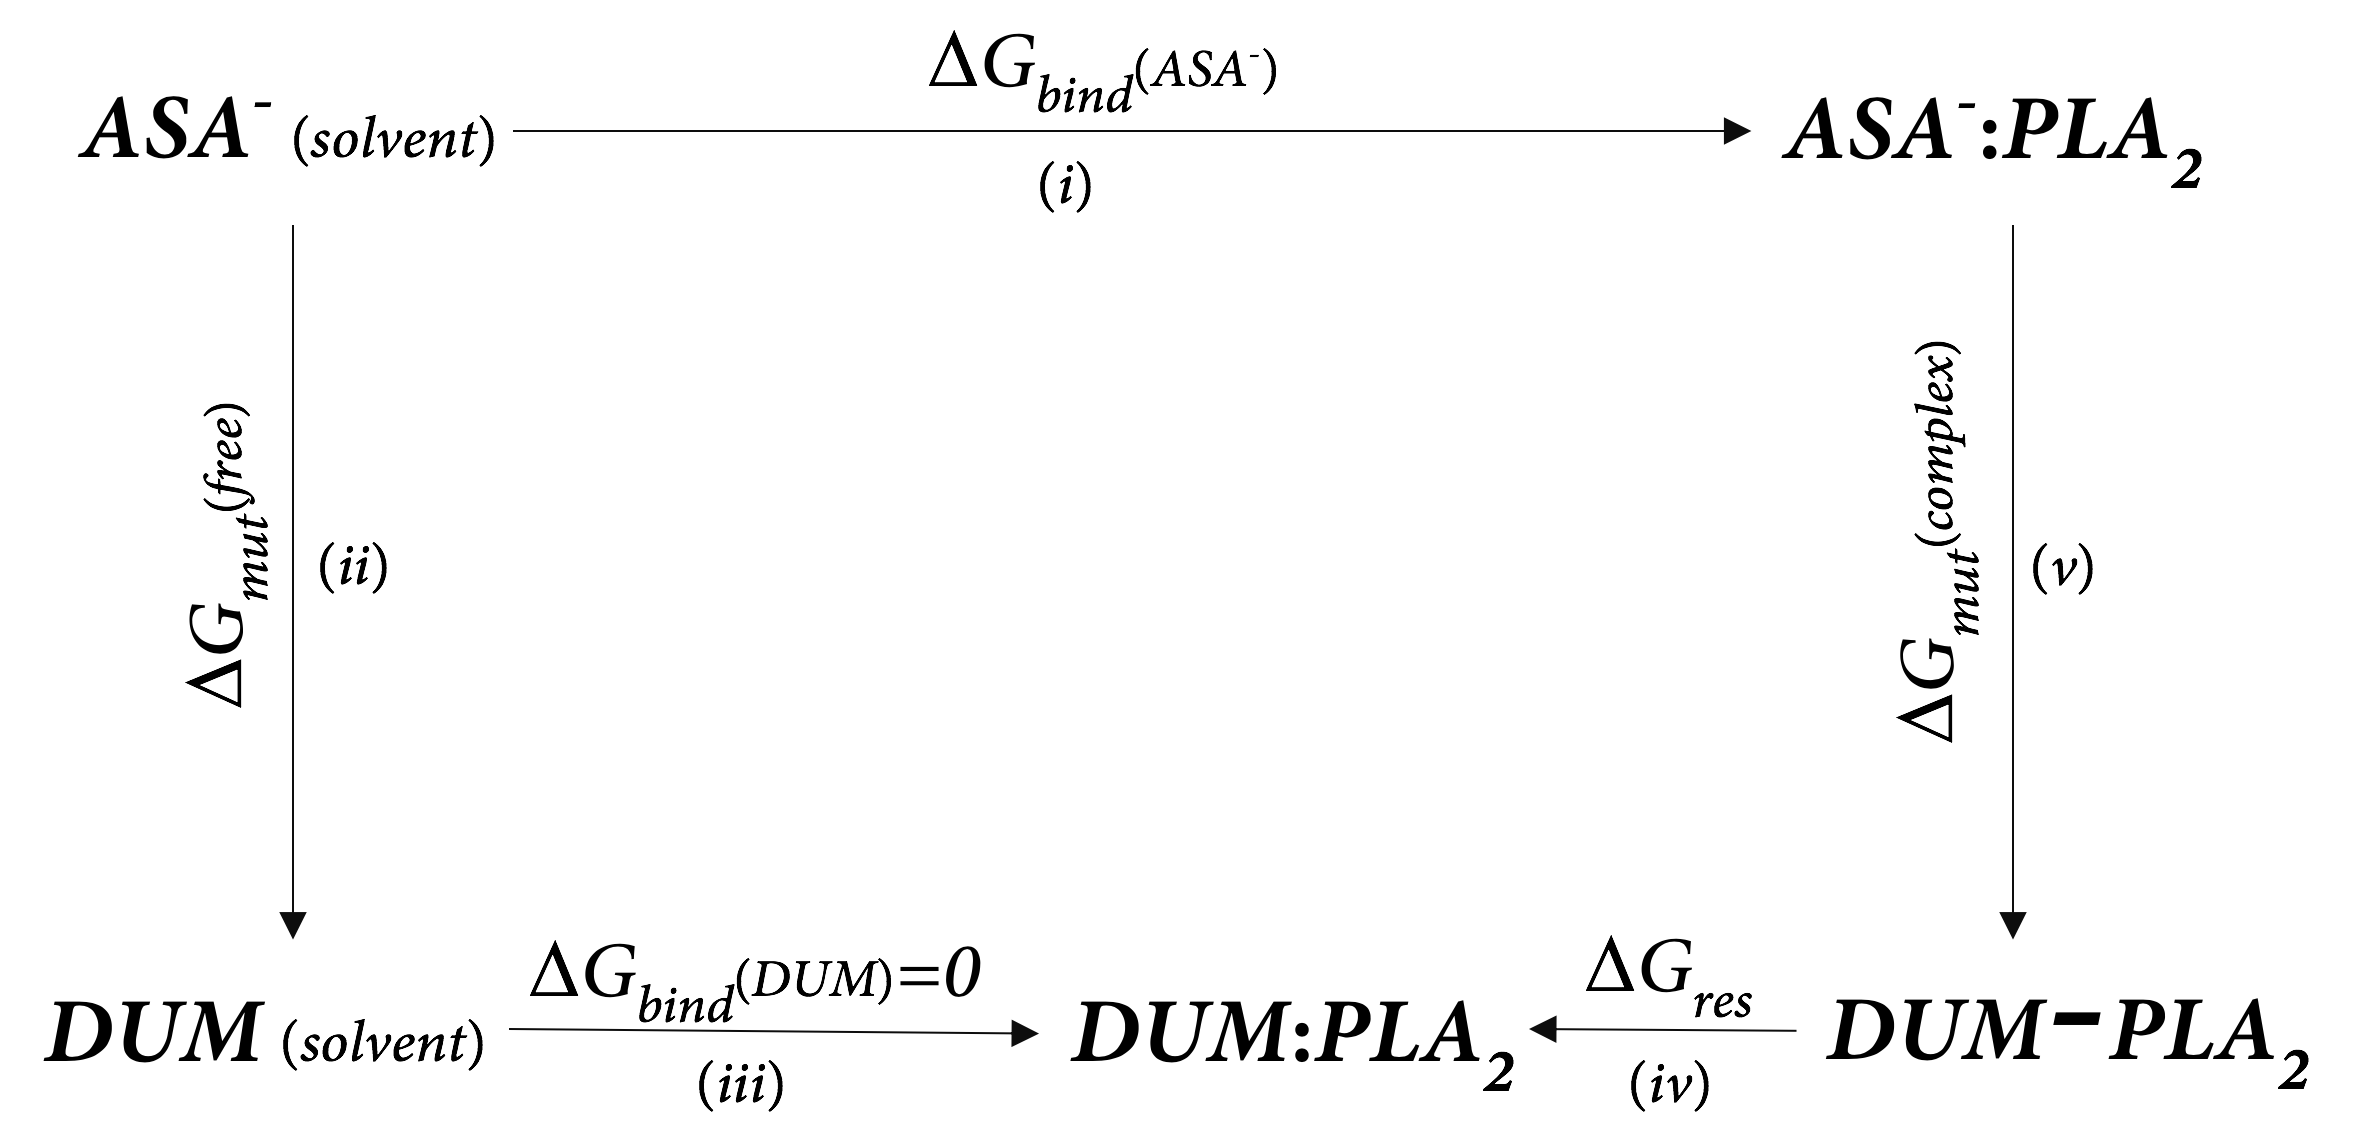
\includegraphics[scale=0.21]{../05_tutorial_02/figures/TC_ASA.png}
    \caption{Thermodynamic cycle for the calculation of the standard binding free energy of aspirin (ASA$^-$) binding to the protein phospholipase A$_2$ (PLA$_2$). ASA$^-$ is turned into a non-interacting dummy molecule (DUM), both in its complexed state (\textit{v}) and free in solution (\textit{ii}). The free energy of DUM binding to PLA$_2$ is zero (\textit{iii}). An intermediate state (DUM-PLA$_2$) is introduced by linking both binding partners with a harmonic distance restraint. The free energy contribution of this restraint can be calculated analytically (\textit{iv}) via equation \ref{disres}. The free energy differences of branches (\textit{ii}) and (\textit{v}) are determined via (extended) thermodynamic integration (TI), enabling the calculation of the standard binding free energy (\textit{i}).}
    \label{TC_ASA}
\end{figure}
%
In this tutorial we will calculate the standard binding free energy of aspirin (ASA) to the protein phospholipase A$_2$ (PLA$_2$) using the DDM and extended-thermodynamic interaction (X-TI)~\cite{X_TI}. 
For an application of X-TI and corrections of net-charge changes in current research see e.~g. Ref.~\cite{Ohlknecht_2020b}.

\subsubsection{Simulation setup}
Preparation of topologies and coordinate files, energy minimization, solvation in SPC water and the addition of counter ions as well as the setup of equilibrations and simulations can be performed in analogy to tutorial 1. The Cartesian coordinates for the enzyme phospholipase A$_2$ with bound acetyl salicylic acid (ASA) can be obtained from the Protein Databank with accession code 1OXR~\cite{Singh2005}.
The final equilibrated structures, \texttt{eq\_ASA\_Na\_7.cnf} and \texttt{eq\_PLA2\_ASA\_Ca\_2Na\_7.cnf}, are in subdirectories \texttt{eq/eq\_ASA} and \texttt{eq/eq\_PLA2\_ASA} of the directory \texttt{t\_02}. 

\subsubsection{Perturbation topology}
Go into the subdirectory \texttt{topo}. The topologies for the ligand (\texttt{ASA.top}) and the protein (\texttt{PLA2.top}) are already prepared. You can also find the combined topologies with sodium counter ions and a calcium ion that is important for the ligand binding (\texttt{ASA\_Na.top} and \texttt{PLA2\_ASA\_Ca\_2Na.top}). For ligand decoupling, the topology for ASA in the decoupled state (\texttt{DUM.top}) was generated by changing the integer atom code (\texttt{IAC}) to 22 corresponding to dummy type for all the atoms and setting all the charges to 0. The program \texttt{make\_pt\_top} can convert topologies from state A and B into a perturbation topology. The \texttt{PERTATOMPARAM} block lists all atoms with their respective force field parameters that will be alchemically perturbed during the simulation. 

\subsubsection{Distance restraints}
Distance restraints are introduced for the calcium ion to keep it bound in the active site. For this a distance restraint specification file \texttt{disres.dat} is set up in subdirectory \texttt{eq} containing the following block.
\begin{lstlisting}[columns=flexible]
DISTANCERESSPEC
# DISH  DISC
  0.1   0.153
# i     j  k  l  type i    j  k  l  type r0     w0    rah
  1208  0  0  0  0    309  0  0  0  0    0.223  1.0   0
  1208  0  0  0  0    321  0  0  0  0    0.235  1.0   0
  1208  0  0  0  0    339  0  0  0  0    0.246  1.0   0
  1208  0  0  0  0    489  0  0  0  0    0.255  1.0   0
  1208  0  0  0  0    490  0  0  0  0    0.248  1.0   0
END
\end{lstlisting}
The restraint is defined between the calcium ion and 5 atoms of residues coordinating the ion (3 amide oxygens and 2 carboxylate oxygens). \texttt{type} \texttt{0} is referring to explicit/real atoms. \texttt{r0} is the distance between two atoms in nm. The restraint is defined with a weight factor \texttt{w0} of 1 by which the distance restraint interaction term \texttt{CDIR} of the \texttt{DISTANCERES} block in the \texttt{imd}-file gets multiplied (force constant). The parameter \texttt{rah} controls the form and dimension of the restraint, here it is set to zero which corresponds to a full harmonic potential in $x$, $y$, $z$ dimensions. Parameters \texttt{DISH} and \texttt{DISC} are the hydrogen-carbon and carbon-carbon distances, respectively. GROMOS can also apply distance restraints on virtual or pseudo atoms by setting the appropriate type and a specification of additional atoms \texttt{j}, \texttt{k} and \texttt{l}. \\

To keep the ligand within the active site when getting decoupled, we gradually turn on a harmonic distance restraint simultaneously to the perturbation. Go into the subdirectory \texttt{DDM/md\_TI} where you will find the \texttt{disres.dat} file which contains an additional block.
\begin{lstlisting}
PERTDISRESSPEC
# DISH  DISC
0.1  0.153
# i j   k   l type i    j    k    l type n m Ar0  Aw0  Br0  Bw0 rah
 21 211 264 529 -1 1195 1199 1203 0 -1   0 0 0.0  0.0  0.0  1.0 0
END 
\end{lstlisting}

The distance restraint is defined between the centre of geometry (\texttt{type} \texttt{-1}) of 4 backbone atoms (\texttt{i}, \texttt{j}, \texttt{k} and \texttt{l}) of PLA$_2$ around the active site and the centre of geometry of 3 atoms of the ligand's benzene ring with a distance of zero (\texttt{A\_r0=B\_r0=0}). At state A the restraint is turned off (\texttt{A\_w0=0}), while at state B the restraint is retained with a weight factor of 1 (\texttt{B\_w0=1}). Parameters \texttt{n} and \texttt{m} control hidden 
restraints~\cite{Christen}. Parameters \texttt{DISH} and \texttt{DISC} are not relevant for the centre of geometry and this type of pseudo atoms.

\subsubsection{Extended-thermodynamic integration simulation}
The thermodynamic integration approach uses the coupling parameter $\lambda$, which defines the system as a linear combination of the two end-states~\cite{kirkwood_TI}. The coupling parameter approach formulates the Hamiltonian of the system dependent on $\lambda$ by interpolating between the two states (scaling of force-field parameters). \\

\begin{align}
\label{equ:ext_ti}
V_{\text{nb}}(r_{ij},\lambda) = (1-\lambda)^n V^{\text{A}}(r_{ij},\lambda) + \lambda^n V^{\text{B}}(r_{ij},1-\lambda)
\end{align}
with
\begin{align}\begin{split}
V^{\text{X}}(r_{ij},\lambda) = \frac{C_{12}^{\text{X}}}{(\alpha_{\text{lj}}\lambda^2 C_{126}^{\text{X}} + r_{ij}^6)^2} - \frac{C_{6}^{\text{X}}}{\alpha_{\text{lj}}\lambda^2 C_{126}^{\text{X}} + r_{ij}^6} + \\
 \frac{q_i^{\text{X}} q_j^{\text{X}}}{4 \pi \epsilon_0} \left \lbrack \frac{1}{(\alpha_{\text{crf}}\lambda^2 + r_{ij}^2)^{1/2}} - \frac{1/2 C_{\text{rf}}r_{ij}^2}{(\alpha_{\text{crf}} \lambda^2 + R_{\text{rf}}^2)^{3/2}} - \frac{1 - 1/2C_{\text{rf}}}{R_{\text{rf}}} \right \rbrack
\end{split}\end{align}

\noindent where $C_{6}^{\text{X}}$, $C_{12}^{\text{X}}$, $q_i^{\text{X}}$ and $q_j^{\text{X}}$ are the Lennard-Jones parameters and partial charges for state X (A or B). $r_{ij}$ is the distance between particles $i$ and $j$, $C_{\text{rf}}$ and $R_{\text{rf}}$ are parameters of the electrostatic reaction field assumed outside the cutoff sphere \cite{Tironi1995}. 
$\alpha_{\text{crf}}$ and $\alpha_{\text{lj}}$ are soft-core parameters \cite{Beutler1994}. 

Go into the subdirectory \texttt{md\_TI}. The input files \texttt{md\_TI\_ASA\_Na.imd} and \texttt{md\_TI\_PLA2\_ASA\_Ca\_2Na.imd} contain two additional blocks that are relevant for the free energy calculations using X-TI integration. The \texttt{PERTURBATION} block controls the alchemical perturbation 
\begin{lstlisting}
PERTURBATION
#     NTG   NRDGL    RLAM   DLAMT 
        1       0     0.0     0.0 
#  ALPHLJ   ALPHC    NLAM  NSCALE 
      1.0     1.0       1       0 
END
\end{lstlisting}
\texttt{NTG} turns on the perturbation to calculate $\partial\mathcal{H}/\partial\lambda$ and \texttt{RLAM} is the initial value for $\lambda$. The initial value of $\lambda$ could also be read from the configuration when setting \texttt{NRDGL=1}. \texttt{RLAM} will be adjusted for several different $\lambda$ points using the jobs file \texttt{md\_TI.jobs}. \texttt{DLAMT} controls the increase of $\lambda$ with time. The parameters \texttt{ALPHLJ} and \texttt{ALPHC} are the soft-core parameters for Lennard-Jones ($\alpha_{\text{lj}}$) and Coulomb ($\alpha_{\text{crf}}$) interactions, respectively. \texttt{NLAM} controls the power dependence of the $\lambda$ coupling ($n$ in eq. \ref{equ:ext_ti}) and \texttt{NSCALE} the use of interaction scaling for complete energy groups.  

The \texttt{PRECALCLAM} block is relevant for the pre-calculation of intermediate non-simulated $\lambda$-points during the simulation as extension to standard TI. 
\begin{lstlisting}
PRECALCLAM
# NRLAM   MINLAM   MAXLAM
     81        0        1
END
\end{lstlisting}
With the settings in the above block, the energies and derivatives with respect to $\lambda$ will be calculated on-the-fly at 81 points ranging from $\lambda$=0 to $\lambda$=1, which results in $\lambda$-steps of 0.0125.


%%for PLA2-ASA with disres and new gromos binary
The simulation is defined in the jobs file \texttt{md\_TI.jobs}. Simulations will be performed at 11 equally spaced $\lambda$-points between $\lambda$=0 and $\lambda$=1 for 5 ns each in case of the complexed system, where ASA is bound to PLA$_2$. This system also requires the perturbed distance restraint. The simulations of ASA free in solution will also be performed at 11 $\lambda$-points each for 0.5 ns.   
Note that this tutorial can also be carried out using standard TI, in which case the \texttt{PRECALCLAM} block is not required. 
The choice of 11 equally spaced $\lambda$-points is typically a reasonable start, but it is recommended to adjust the number of points and the spacing according to the curvature and error estimates of $\partial\mathcal{H}/\partial\lambda$. 
In X-TI, adjustment is often not necessary, even fewer points are sufficient in some cases, but for standard TI usually more than 11 $\lambda$-points are needed. 
Therefore, we strongly recommend to use the \texttt{PRECALCLAM} block and take advantage of the pre-calculation of intermediate non-simulated $\lambda$-points and subsequent reweighting.
To run the two simulations, copy the argument files required by the \texttt{mk\_script} program into the two directories \texttt{md\_TI\_ASA} and \texttt{md\_TI\_PLA2\_ASA}, respectively, and adapt the paths before generating the job files with the \texttt{mk\_script} program and submitting the jobs to a cluster. If you prefer to continue directly, you will find the necessary energy and free energy trajectories in the subdirectories \texttt{L\_*}.

\subsubsection{Free energy analysis}
The free energies can be determined via extended-thermodynamic integration (X-TI)~\cite{X_TI} or the Bennett acceptance ratio (BAR) method~\cite{bar}. The raw data for both methods can be extracted from the energy and free energy trajectory files using the gromos++ program \texttt{ext\_ti\_ana}. 

Go into the subdirectory \texttt{DDM/ana\_TI/ana\_TI\_ASA} and run the program \texttt{ext\_TI\_ana} via the bash-script by typing
\begin{lstlisting}
$ ./ext_ti_ana_bar.sh
\end{lstlisting}
%
X-TI requires the pre-calculation of free energies at non-simulated points. Free energy derivatives at requested non-simulated $\lambda_{\text{P}}$ values can be reweighted to obtain ensemble averages for $\lambda_{\text{P}}$ from simulated $\lambda_{\text{S}}$ points. The predictions from multiple simulations at $\lambda_{\text{S}}$ points can be merged into a single TI profile by a linear reweighting scheme using the program \texttt{ext\_TI\_merge}. 
Run the program via the bash-script by typing
\begin{lstlisting}
$ ./ext_ti_merge.sh
\end{lstlisting}
%
The program calculates the integral of the final TI-curve using the trapezoidal rule in order to obtain the free energy estimate. The results of X-TI for both systems, ASA and PLA2\_ASA, are shown in Figure~\ref{TI_ASA}.  


BAR estimates free energies from the free energy differences between two adjacent $\lambda$ points $i$ and $j$, using
\begin{align}
\Delta G(\lambda_i \rightarrow \lambda_j) 
     = k_{\text{B}} T \ln \frac{\langle f(E(\lambda_i) - E(\lambda_j) + C)\rangle_{\lambda_j}}
          {\langle f(E(\lambda_j)-E(\lambda_i) - C )\rangle_{\lambda_i}}  + C
\end{align}
with
\begin{align}
f(x) = \frac{1}{1+\exp(x/k_{\text{B}} T)}
\end{align}
$C$ is determined iteratively to ensure that the two ensemble averages
from $\lambda_i$ and $\lambda_j$ are identical. To calculate error estimates, a
bootstrap sampling can be conducted. Run the program \texttt{bar} via
the bash-script by typing
\begin{lstlisting}
$ ./bar.sh 
\end{lstlisting}
%
BAR is computationally more efficient and converges relatively fast compared to regular TI. The efficiency of X-TI is comparable with the added advantage of a direct visualization of the entire free energy profile~\cite{Maurer}.

\begin{figure}[H]
    \centering
    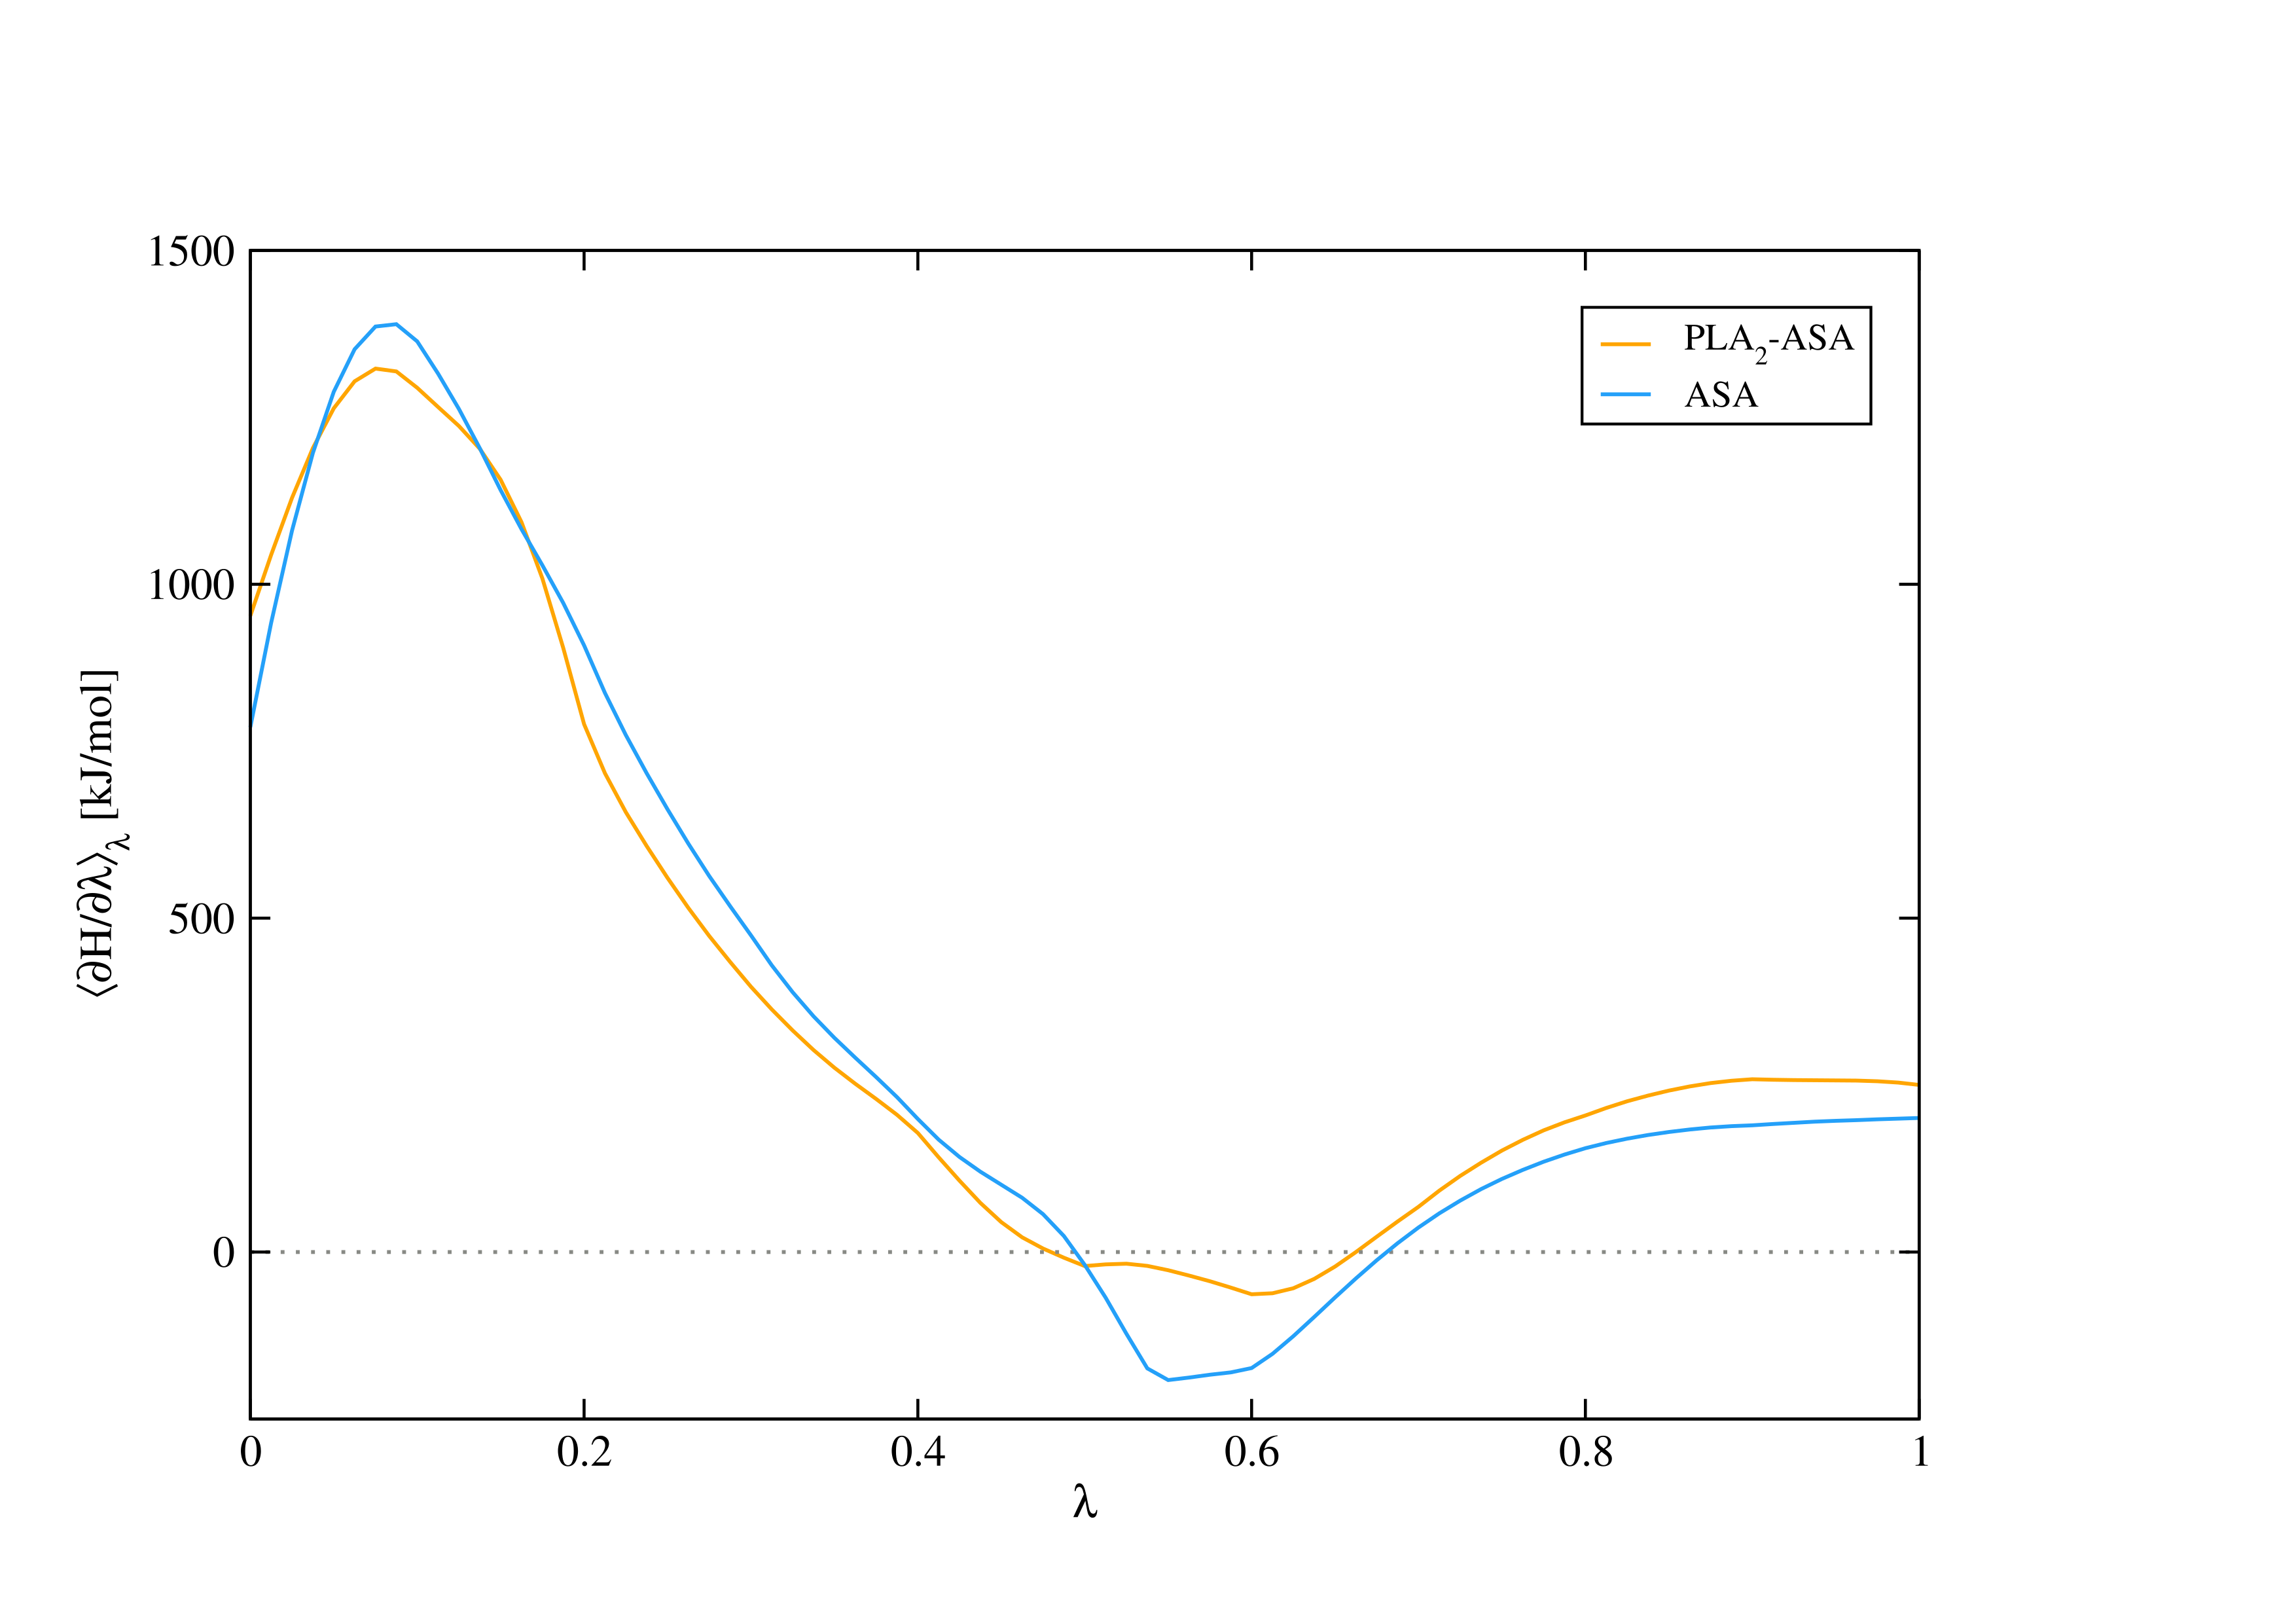
\includegraphics[scale=0.3]{../05_tutorial_02/figures/ana_TI.png}
    \caption{The reweighted property $\left<\frac{\partial\mathcal{H}}{\partial\lambda}\right>$ for $\lambda$=0 to $\lambda$=1 for both systems ASA and PLA$_2$\_ASA.}
    \label{TI_ASA}
\end{figure}

\subsubsection{Thermodynamic cycle}
The free energy of binding is determined according to the thermodynamic cycle shown in Figure~\ref{TC_ASA} as
\begin{align}\begin{split}
& \Delta G_{\text{bind}}(\text{ASA}^-)= \\ 
& \Delta G_{\text{mut}}(\text{free})+\Delta G_{\text{bind}}(\text{DUM})-\Delta G_{\text{res}}-\Delta G_{\text{mut}}(\text{complex})
\end{split}\end{align}
%
The free energy associated with the removal of the restraint ($\Delta G_{\text{res}}$) for a dummy particle can be calculated analytically, including a standard state correction~\cite{Roux, Boresch}: 
\begin{align} \label{disres}
    \Delta G_{\text{res}} = -k_{\text{B}}T \ln\frac{V^{\circ}}{\Big(2\pi k_{\text{B}}T/K\Big)^{3/2}}
\end{align}
where $K$ is the force constant of the harmonic distance restraint and $V^{\circ}$ is the accessible solution volume corresponding to the standard-state definition. For a molar reference concentration it is given by $V^{\circ}=1.661$~nm$^3$.
Equation \ref{disres} corrects for restricted mobility and can be derived from the partition function associated with the restraining potential energy function, 
given that the restraint is so strong that the integration volume can be extended to the entire space~\cite{Gebhardt2016}.

\subsubsection{Correction terms for net-charge changes}
Due to finite box sizes, periodic boundary conditions and
simplifications in the calculations of the electrostatic interactions,
the calculated free energies are artifacted. In the following
paragraphs, we will refer to these energies as raw free energies. We
will quantify and correct these artifacted components using a
free energy correction $\Delta G_{\text{cor}}$ to yield methodology-independent
values $\Delta G$ as
\begin{align}
    \Delta G = \Delta G_{\text{raw}} + \Delta G_{\text{cor}}
\end{align}
%
Analogous to Reif and Oostenbrink~\cite{Reif2014}, $\Delta G_{\text{cor}}$ is a
combination of multiple free energy corrections for a spurious
solvent-polarization ($\Delta G_{\text{pol}}$), the impracticality
of
calculating the zero of the potential under periodic boundary
conditions using discrete solvent molecules ($\Delta G_{\text{dsm}}$) and
artifacted direct interactions between the ligand and the host
molecule ($\Delta G_{\text{dir}}$). The free energy correction is calculated
as
\begin{align} \label{equ:corrected_free_energy}
  \Delta G_{\text{cor}} = \Delta G_{\text{pol}} + \Delta G_{\text{dir}} + \Delta G_{\text{dsm}}
\end{align}
%
These three correction terms will be calculated in the following
paragraphs. A general scheme about the calculation of the corrections
based on $\lambda$-generated trajectories can be found in
Figure~\ref{fig:correction_scheme}~\cite{Ohlknecht2020}. 
Note that within this tutorial, only the information needed for the
practical part is provided, further details about the theory can be
found elsewhere~\cite{ReifBook2011,Kastenholz2006_I,Reif2014}. The set
of the three correction terms needs to be calculated for both branches of
the thermodynamic cycle. Have a look into the directory
\texttt{corrections}. It contains subdirectories for Aspirin free in
solution and the complex of Phospholipase A2 with Aspirin. The
correction procedure will only be explained for Aspirin free in
solution, the procedure for the complex is similar. Go into the
directory \texttt{corrections/ASA}. First, we need to create a set of
topologies for intermediate states. These topologies will have full,
unperturbed VdW parameters but charges that scale with $\lambda$.  Go
further into the subdirectory \texttt{correction\_topologies}. The
python script \texttt{interpolate\_topocharges.py} takes three input
parameters: topologies at states A and B and a specific
$\lambda$-value. A new topology with charges that correspond exactly
to the given $\lambda$-value is written out. All other parameters
remain unperturbed and are taken from topology A. We do not have to use
it directly but can use the bash script
\texttt{do\_interpolate\_topocharges.bash} instead. It creates six
topologies at equidistant $\lambda$-points. These will be used for the
individual correction terms explained in the following paragraphs.

\begin{figure}[H]
    \centering
    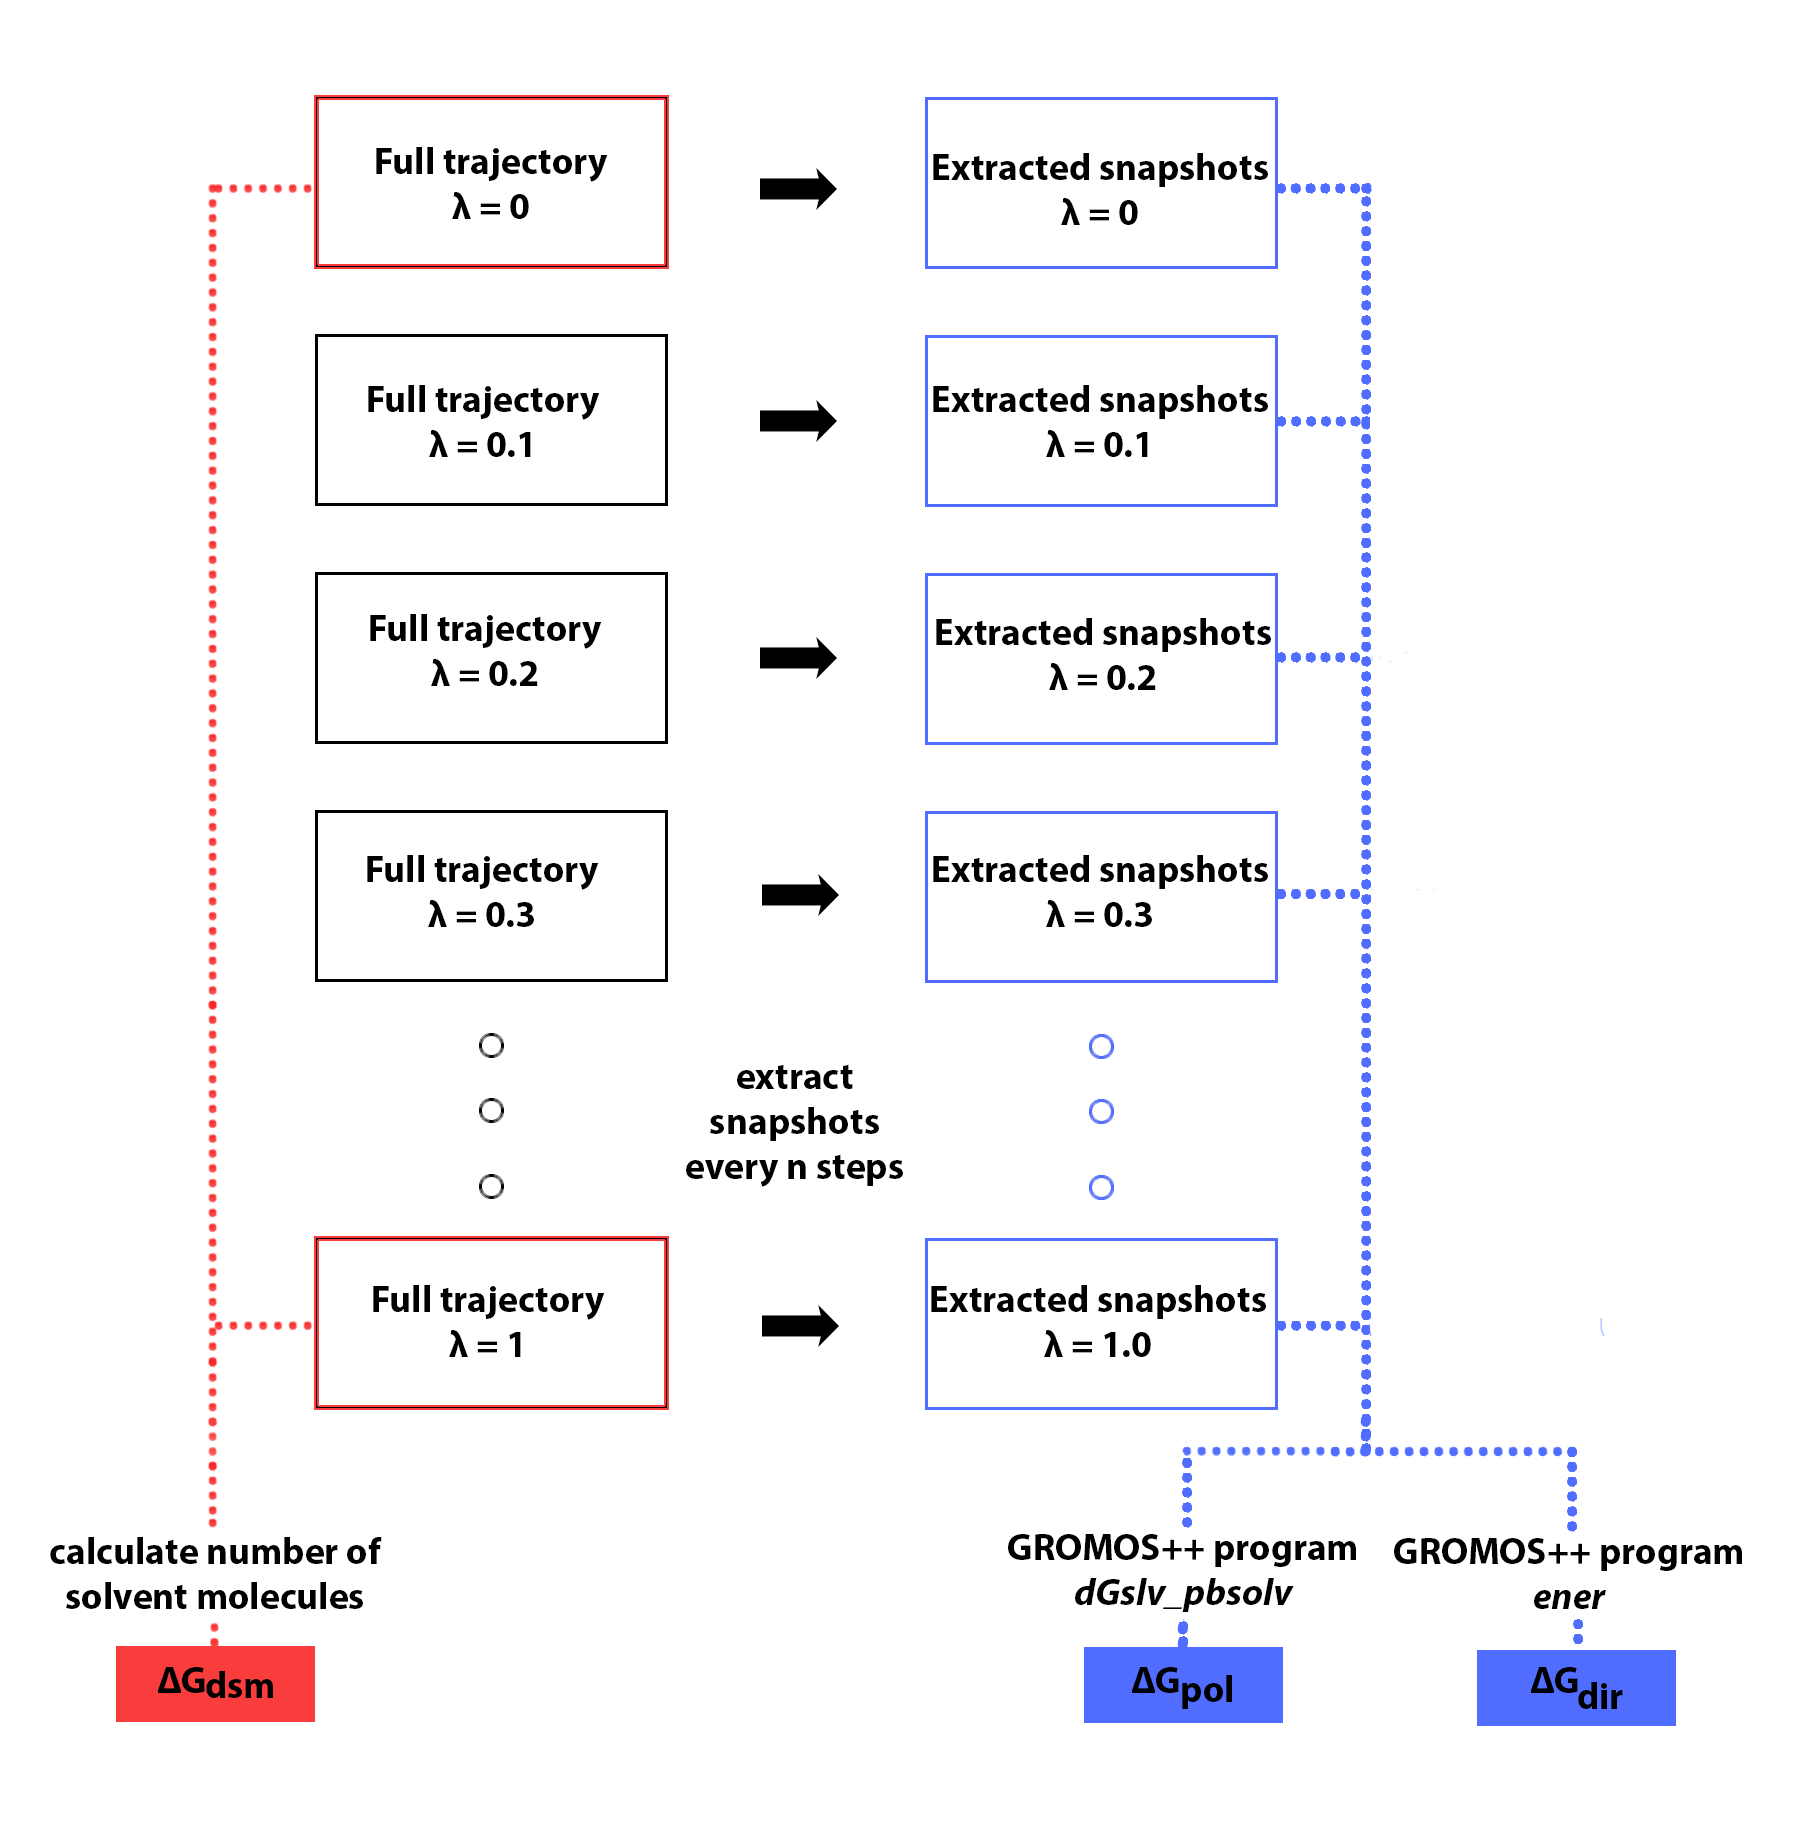
\includegraphics[scale=0.14]{../05_tutorial_02/figures/general_application_corrections.png}
    \caption{Schematic representation of the corrections. $\Delta G_{\text{dsm}}$ is
      calculated over full trajectories of the end states (however, if one of the end states has zero charges, it can be skipped). $\Delta G_{\text{pol}}$ and $\Delta G_{\text{dir}}$ are both calculated on individual snapshots
      only. In this tutorial, only the final snapshots of 6 chosen $\lambda$-points are used for these calculations.}
    \label{fig:correction_scheme}
\end{figure}


\subsubsection{Solvent polarisation}
First, we calculate the correction estimate $\Delta G_{\text{pol}}$ for the
spurious solvent polarisation. We will use a set of
continuum-electrostatics calculations on configurations extracted from
trajectories that were sampled at different $\lambda$ points. For each of
these configurations, the electrostatic potential at the atom sites of the
Aspirin molecule will be calculated twice - using a cutoff scheme with
a reaction-field contribution under periodic boundary conditions and
using full Coulombic charges under non-periodic boundary
conditions. The integrated differences between both
potentials will give an estimate of $\Delta G_{\text{pol}}$, which can be directly
applied to the raw free energies that were calculated in the
simulation. Note that for the sake of simplicity, in this tutorial we
will use only the last configurations of six $\lambda$-generated
trajectories. However, when used for ``real'' research questions, a
more complete set of configurations should be analysed in order to achieve
more reliable results.

Go into the subdirectory \texttt{corrections/ASA/dGpol}. It
contains argument files for the GROMOS++ program
\texttt{dGslv\_pbsolv}. There are six argument files for six different
$\lambda$ points.
% and one additional argument file that uses a snapshot that was generated with full charges but is re-analyzed with zero charges. 
Since the continuum-electrostatics calculations are
computationally demanding, the output files are already
provided. However, if you prefer to run the continuum-electrostatics
calculations yourself, you can run them by typing
\begin{lstlisting}
$ dGslv_pbsolv @f dGslv_pbsolv_L_0.0.arg > dGslv_pbsolv_L_0.0.out
$ dGslv_pbsolv @f dGslv_pbsolv_L_0.2.arg > dGslv_pbsolv_L_0.2.out
...
$ dGslv_pbsolv @f dGslv_pbsolv_L_1.0.arg > dGslv_pbsolv_L_1.0.out
\end{lstlisting}
%$ dGslv_pbsolv @f ASA_Na_L_0.0_no_charges.arg > ASA_Na_L_0.0_no_charges.out
%
Let's have a look at one of the output files. It contains four rows for
the individual atoms of the charged acetyl group
of the Aspirin molecule. There are several
columns. Next to basic information for the individual atoms, there are
six columns with potentials created under non-periodic boundary
conditions in solvation (NPBC\_SLV), non-periodic boundary conditions
in vacuum (NPBC\_VAC), periodic boundary conditions in solvation
(PBC\_SLV), periodic boundary conditions in vacuum (PBC\_VAC), a fast
Fourier transform result for the lattice-summation method under
periodic boundary conditions (FFT\_LS\_PBC) and a fast Fourier
transform result for the reaction-field method under periodic boundary
conditions (FFT\_RF\_PBC).  The potential that has to be integrated
over $\lambda$ reads (NPBC\_SLV - NPBC\_VAC) - (PBC\_SLV - PBC\_VAC) -
(FFT\_LS\_PBC - FFT\_RF\_PBC). Note that the last term has to be used
only if a cutoff scheme with reaction field contribution was applied
in the simulation. You can simply use the script
\texttt{integrate.py}. Type
\begin{lstlisting}
$ ./integrate.py
\end{lstlisting}
We are interested in the result NPBC - PBC, which is the correction term $\Delta G_{\text{pol}}$.
%12.3 kJ/mol. 

\subsubsection{Direct ligand-protein interactions}
In the actual MD simulation, the interaction between the ligand and
the protein atoms was calculated by a cutoff scheme with a reaction
field contribution. A correct scheme would involve no cutoff and
purely Coulombic interactions. $\Delta
G_{\text{dir}}$ accounts for the difference between the simulated and the
real case. Note that in order to minimize the dependence of the
correction terms on the conformations of the molecules the same
configurations have to be used for $\Delta
G_{\text{dir}}$ that were used for the calculations of $\Delta
G_{\text{pol}}$. Go into the subdirectory
\texttt{corrections/ASA/dGdir}. It contains argument files for the
GROMOS++ program \texttt{ener}. There are 12 argument files for six
different $\lambda$-points,
one for Coulombic interactions under non-periodic boundary conditions
(NPBC) and one for Coulomb/Reaction-field interactions under periodic
boundary conditions (PBC). You can use the provided output files or
generate them yourself by typing
\begin{lstlisting}
$ ener @f ener_PBC_L_0.0.arg > ener_PBC_L_0.0.out
$ ener @f ener_NPBC_L_0.0.arg > ener_NPBC_L_0.0.out
$ ener @f ener_PBC_L_0.2.arg > ener_PBC_L_0.2.out
...
$ ener @f ener_NPBC_L_1.0.arg > ener_NPBC_L_1.0.out
\end{lstlisting}
%
We are interested in the integrated energies NPBC-PBC. You can do it
yourself or use a provided Python script. Simply type
\begin{lstlisting}
$ ./integrate.py 
\end{lstlisting}
The integrated result is the correction term $\Delta G_{\text{dir}}$. %should be around -9.1 kJ/mol.

\subsubsection{Potential from discrete solvent molecules}
Another artifact stems from the impossibility of calculating the
absolute zero potential in a periodic simulation box and the
convention to average the solvent-generated potential over the
exterior and the interior of the solvent molecules. As a consequence,
the calculated potential differs from the ``real'' potential by an
offset. For a rigid solvent model with a single van der Waals
interaction site and any scheme relying on molecular-cutoff truncation
based on this specific site, it can be shown that this offset is
related to the quadrupole moment trace of the solvent model used. The
free energy correction is furthermore proportional to the
water-molecule density inside the box (LS - lattice summation schemes)
or within the cutoff radius (cutoff schemes with reaction-field
correction - RF) and reads
\begin{equation}
  \Delta G_{\text{dsm}}(\text{LS}) = -N_{\text{A}} (6 \epsilon_0)^{-1} \gamma_{\text{s}} \Delta Q N_{\text{S}} V_{\text{B}}^{-1}
\end{equation}
for the LS scheme and
\begin{equation} \label{equ:dsm}
  \Delta G_{\text{dsm}}(\text{RF}) = -N_{\text{A}} (6 \epsilon_0)^{-1} \frac{2 (\epsilon_{\text{RF}}-1)}{2\epsilon_{\text{RF}}+1} \gamma_{\text{s}} \sum_{i=1}^n \Delta q_i \left\langle N_{\text{S}}(R_{\text{C},i})\right\rangle V_{\text{C}}^{-1}
\end{equation}
for the RF scheme, where $N_{\text{A}}$ is the Avogadro constant, $\epsilon_0$
is the vacuum dielectric permittivity, $\epsilon_{\text{RF}}$ is the (relative)
reaction-field dielectric permittivity, $\Delta Q$ is the net-charge
change in the system, $\Delta q_i$ is the net-charge change of the perturbed atom $i$, $N_{\text{S}}$ is the number of solvent molecules in the
box, $\left\langle N_{\text{S}}(R_{\text{C},i})\right\rangle$ is the average number of
solvent molecules in the cutoff sphere of the perturbed atom i, $V_{\text{B}}$ is the volume of the
computational box and $V_{\text{C}}$ is the volume of the cutoff
sphere. $\gamma_{\text{s}}$ is the quadrupole moment trace relative to the van
der Waals interaction site. Values for typically used water models can be found in
table \ref{tab:quadrupole_moments}. Hint: the reaction-field permittivity used in the simulations can be found in the \texttt{NONBONDED} block in one of the \texttt{imd} files, parameter \texttt{EPSRF}.

\begin{table}[h]
  \center
  \caption{ Quadrupole-moment traces [e nm$^2$] for typical solvent models}
  \label{tab:quadrupole_moments}
  \begin{tabular}{ l  c  }
    \hline
    \textbf{model} & $\gamma_{\text{s}}$ \\ 
    \hline
    SPC~\cite{Berendsen1981} & 0.008200 \\
    SPC/E~\cite{Berendsen1987} & 0.008476 \\
    TIP3P~\cite{Jorgensen1983} & 0.007641 \\
    TIP4P~\cite{Jorgensen1983} & 0.009295 \\
    TIP5P~\cite{Mahoney2000} & 0.002054 \\
    ST2~\cite{Stillinger1974} & 0.001754 \\
    \hline
  \end{tabular}
\end{table}
%
Go into the subdirectory \texttt{corrections/ASA/dGdsm}. First, we need
to calculate the average number of water molecules in the cutoff
sphere that was used in the simulation. We will calculate this number
using a radial distribution function (rdf) over the trajectory that
was generated with full charges on the perturbed atoms. The argument
file for the GROMOS++ program \texttt{rdf} is already provided, 
as is the output file for the case your simulation did not finish yet.
You can run \texttt{rdf} by typing
\begin{lstlisting}
$ rdf @f rdf.arg > rdf.out 
\end{lstlisting}
The output file contains the densities of water particles as function of
the distance of all the perturbed atoms. 
%----------------------------------------------------------------------------------
%To obtain the
%total number of water molecules, these densities need to be integrated
%over the distance and multiplied by the water number density
%$\rho = N/V_{\text{B}}$ in the simulation box. The latter can be found by looking
%into one of the configuration files - the POSITION block contains the
%number of solvent molecules and the GENBOX block provides the box
%dimensions.  The integral over the rdf can be calculated using the
%provided Python script. You can simply run it by
%typing %The calculated water number density in the box should be roughly 32.4.
%\begin{lstlisting}
%$ ./integrate.py
%\end{lstlisting}
%%The calculated total amount of water molecules in the cutoff sphere
%%should be about 370.
%Equation \ref{equ:dsm} then gives the final
%correction term $\Delta G_{\text{dsm}}$. %which should be roughly 77.5 kJ/mol
%---------------------------------------------------------------------------------------------------
To obtain the
total number of water molecules, these densities need to be integrated
over the distance and multiplied by the water number density
$\rho = N/V_{\text{B}}$ in the simulation box. Equation \ref{equ:dsm} then gives the final correction term $\Delta G_{\text{dsm}}$ . You can calculate it by typing
\begin{lstlisting}
$ ./integrate.py
\end{lstlisting} 
This script reads the file \texttt{rdf.out} as well as \texttt{system.info} that contains relevant information about the box size, the cutoff, the correction field and the solvent model.    
Relevant information about the box size can be found by looking
into one of the configuration files - the \texttt{POSITION} block contains the
number of solvent molecules and the \texttt{GENBOX} block provides the box
dimensions.  Settings for the electrostatics can be found in the \texttt{NONBONDED} block in the \texttt{imd} files. 


\subsubsection{Corrected results}
Above, the three correction terms for Aspirin free in solution were
calculated. According to equation \ref{equ:corrected_free_energy}, the
sum of these three correction terms constitutes the total correction
for this branch of the thermodynamic cycle. The same set of correction terms has to be
calculated for the ligand bound to the host (directory \texttt{corrections/PLA2\_ASA}). Both corrections
can be directly added to the raw free energies to yield
methodologically independent results (see table \ref{tab:results}). The final calculated estimate $\Delta G^{\circ}_{\text{bind}} = \Delta G(\text{PLA}_2\_\text{ASA}) - \Delta G(\text{ASA}) = -32.3$ kJ/mol agrees 
quite well with the experimentally determined estimate of $\Delta G_{\text{bind,exp}} = -29.6$ kJ/mol~\cite{Singh2005}.

\begin{table}[h]
  \center
  \caption{ Results from Double Decoupling with corrections. All values are reported in kJ/mol.}
  \label{tab:results}
  \begin{tabular}{ @{}l c@{\phantom{~~}} c c c c@{\phantom{~}} c@{}}
    \hline
    \textbf{System} & $\Delta G_{\text{raw}}$ & $\Delta G_{\text{res}}$ & $\Delta G_{\text{pol}}$ & $\Delta G_{\text{dir}}$ & $\Delta G_{\text{dsm}}$ & $\Delta G$ \\
    \hline
    ASA & -371.2 & - & 12.3 & -9.1 & 77.5 & -290.5 \\
    PLA$_2$\_ASA & -383.2 & 18.2 & -13.3 & 23.4 & 32.1 & -322.8 \\
    \hline
  \end{tabular}
\end{table}
